\documentclass[titlepage]{tufte-book}

\usepackage[runall=true]{pythontex}
\usepackage{amsthm}
\usepackage{amsmath}
\usepackage{amssymb}
\usepackage[pdftex]{graphicx}
\usepackage{epstopdf}
\usepackage{hyperref}
\usepackage{alltt}
\usepackage{listings}
\usepackage{array}
\usepackage{extarrows}
\usepackage{setspace}
\usepackage{tikz}
\usepackage{tikz-qtree}
\usetikzlibrary{calc}
\usetikzlibrary{positioning}
\usepackage{hyperref}
\usepackage{graphviz}
\usepackage{geometry}                % See geometry.pdf to learn the layout options. There are lots.
\usepackage{bashful}
\usepackage{microtype} % Improves character and word spacing

\usepackage{booktabs} % Better horizontal rules in tables

\setkeys{Gin}{width=\linewidth,totalheight=\textheight,keepaspectratio} % Improves figure scaling
\graphicspath{{figures/}}

\usepackage{fancyvrb} % Allows customization of verbatim environments
\fvset{fontsize=\normalsize} % The font size of all verbatim text can be changed here

\newcounter{problem}
\newcounter{total}
\newcommand{\step}[1]{{}
\vspace{4pt} \noindent {\bf \theproblem. }#1\addtocounter{problem}{1}}

\newcommand{\cut}[1]{}

\newcommand{\chili}{\scalebox{.04}{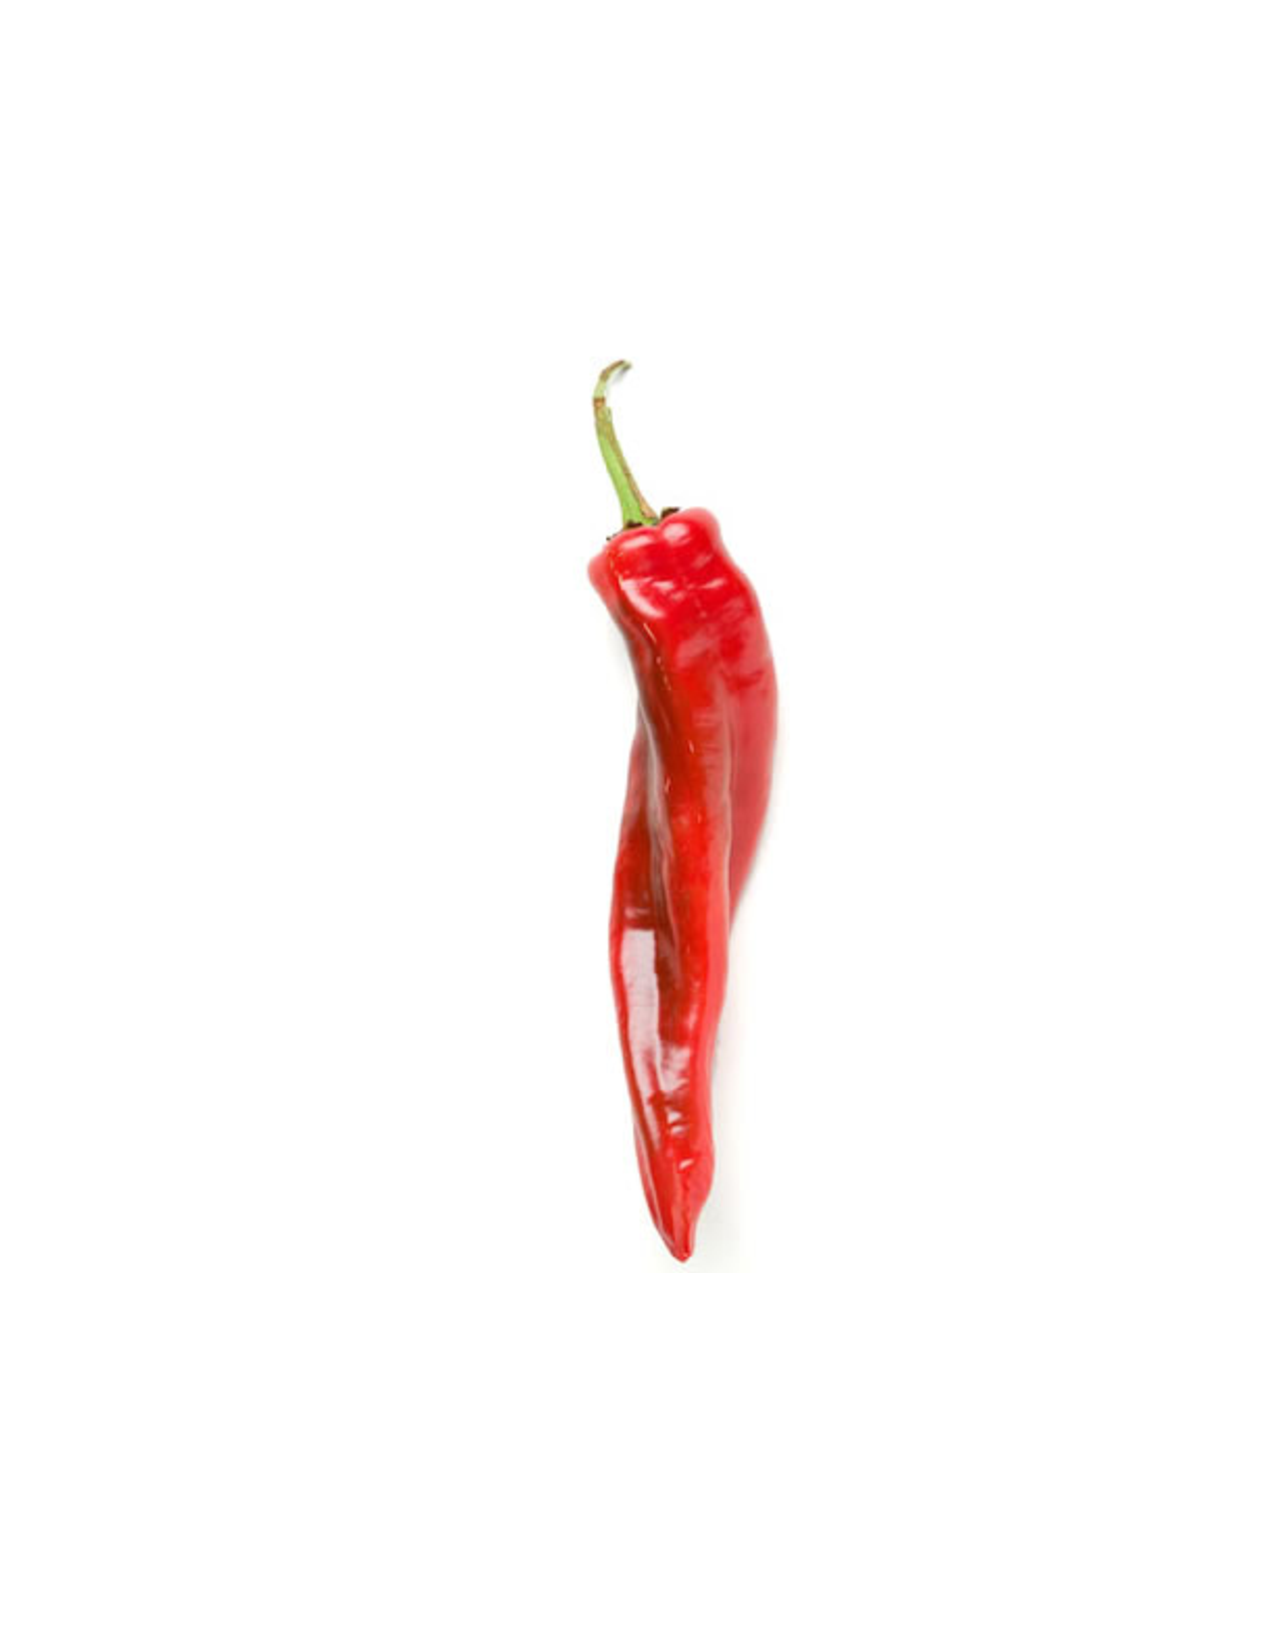
\includegraphics{figures/chili.pdf}}}
\newcommand{\chchili}{{\chili\chili}}
\newcommand{\chchchili}{{\chchili\chili}}

\hypersetup{
urlcolor=blue,
colorlinks=true
}
\usepackage[noline, procnumbered, linesnumberedhidden, boxed]{algorithm2e}

\newcommand{\openepigraph}[2]{ % This block sets up a command for printing an epigraph with 2 arguments - the quote and the author
\begin{fullwidth}
\sffamily\large
\begin{doublespace}
\noindent\allcaps{#1}\\ % The quote
\noindent\allcaps{#2} % The author
\end{doublespace}
\end{fullwidth}
}

\newcommand{\blankpage}{\newpage\hbox{}\thispagestyle{empty}\newpage} % Command to insert a blank page

\usepackage{makeidx} % Used to generate the index
\makeindex % Generate the index which is printed at the end of the document

\renewcommand{\maketitlepage}[0]{%
  \cleardoublepage%
  {%
  \sffamily%
  \begin{fullwidth}%
  ~
  \vspace{11.5pc}%
  \fontsize{36}{40}\selectfont\par\noindent\textcolor{darkgray}{\allcaps{\thanklesstitle}}\\%
~
 \fontsize{12}{18}
 \selectfont\par\textcolor{darkgray}{~~An Excerpt from \href{https://github.com/parrt/msan501}{\textcolor{blue}{MSAN501---Exercises in Computational Analytics}}}\\
\fontsize{36}{40}
\scalebox{.2}{
\includegraphics{figures/msan-logo}}
  \vspace{11.5pc}%
  \fontsize{12}{18}\selectfont\par\indent\textcolor{darkgray}{\allcaps{\thanklessauthor}\\
\indent{\tt parrt@cs.usfca.edu}\\
\href{http://parrt.cs.usfca.edu}{http://parrt.cs.usfca.edu}}%
  \vspace{11.5pc}%
  \fontsize{14}{16}\selectfont\par\noindent\allcaps{\thanklesspublisher}%
  \end{fullwidth}%
  }
  \thispagestyle{empty}%
  \clearpage%
}

\titlecontents{part}% FIXME
    [0em] % distance from left margin
    {\vspace{1.5\baselineskip}\begin{fullwidth}\LARGE\rmfamily\itshape} % above (global formatting of entry)
    {\contentslabel{2em}} % before w/label (label = ``II'')
    {} % before w/o label
    {\rmfamily\upshape\qquad\thecontentspage} % filler + page (leaders and page num)
    [\end{fullwidth}] % after

  \titlecontents{chapter}%
    [0em] % distance from left margin
    {\vspace{1.5\baselineskip}\begin{fullwidth}\Large\rmfamily\itshape} % above (global formatting of entry)
    {\hspace*{0em}\contentslabel{2em}} % before w/label (label = ``2'')
    {\hspace*{4em}} % before w/o label
    {\rmfamily\upshape\qquad\thecontentspage} % filler + page (leaders and page num)
    [\end{fullwidth}] % after

\titlespacing*{\chapter}{0pt}{0pt}{30pt}
\titlespacing*{\section}{0pt}{3.5ex plus 1ex minus .2ex}{2.3ex plus .2ex}
\titlespacing*{\subsection}{0pt}{3.25ex plus 1ex minus .2ex}{1.5ex plus.2ex}

\title{
Launching an AWS\\
Linux Machine
}

% preparatory, introductory, foundations, preliminary, survey
\author{Terence Parr}

\date{} % delete this line to display the current date

%\setcounter{secnumdepth}{0}

\begin{document}

\frontmatter

%----------------------------------------------------------------------------------------

\maketitle % Print the title page

%----------------------------------------------------------------------------------------
%	COPYRIGHT PAGE
%----------------------------------------------------------------------------------------

\newpage
\begin{fullwidth}
~\vfill
\thispagestyle{empty}
\setlength{\parindent}{0pt}
\setlength{\parskip}{\baselineskip}
Copyright \copyright\ \the\year\ Terence Parr

\par\smallcaps{A Bonkers the Cat Production}

\vspace{-65pt}
\scalebox{.35}{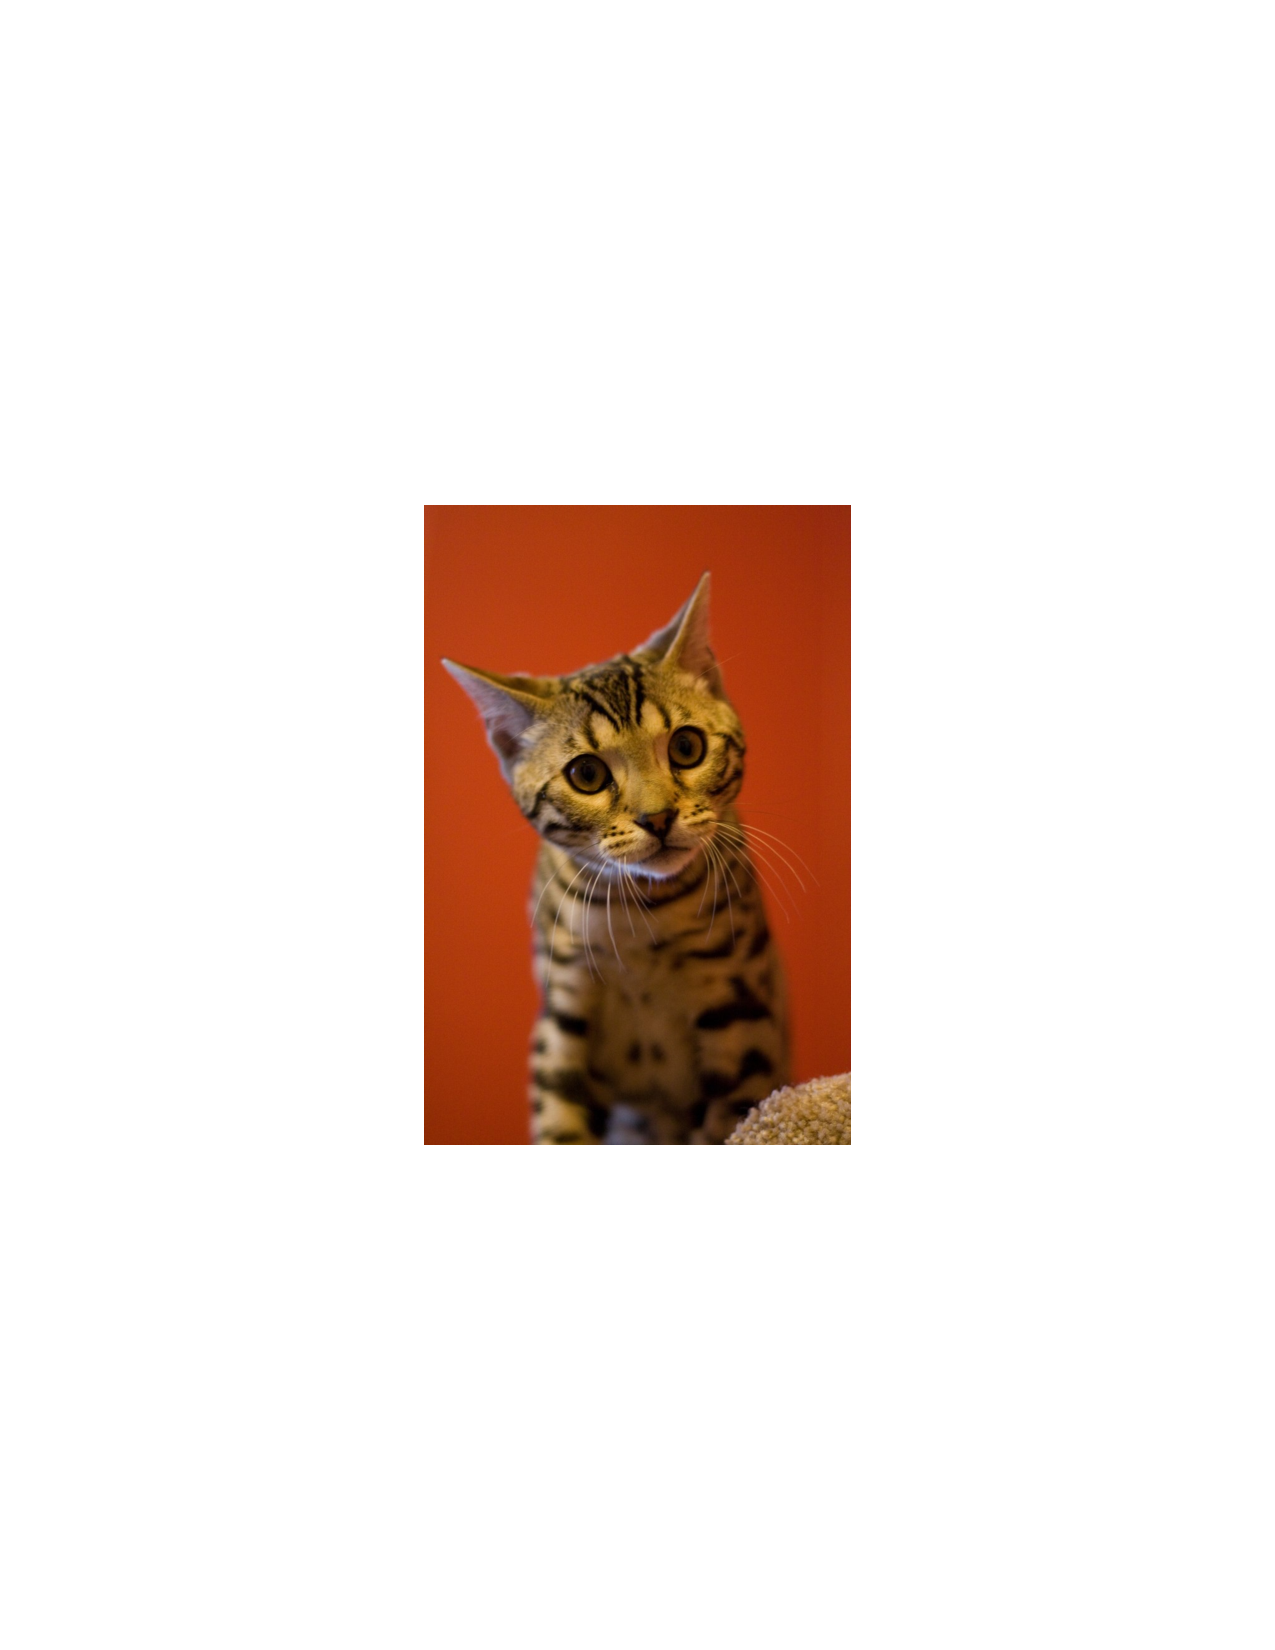
\includegraphics{figures/bonkers}}


\end{fullwidth}

%----------------------------------------------------------------------------------------

\tableofcontents % Print the table of contents

\mainmatter

\chapter{Launching a Virtual Machine at Amazon Web Services}
\label{ch:1}

\setcounter{problem}{1}

\section{Discussion}

\begin{fullwidth}

The goal of this lab is to teach you to create a Linux machine, login, and copy some data to that machine.

\section{Steps}

\step Go to your EC2 dashboard at AWS and click "Launch Instance"; Use the classic Wizard.

\step Select the ``Amazon Linux AMI'' server, which should be the first one. 64bit.

\step Select instance type ``m1.small,'' which should be the second machine type listed. then click continue.

\step Skip over the advanced instance options by clicking continue.

\step Skip over the storage device configuration

\step For the key named "Name", change the value to something like {\em youruserID}-windows or something like that so that you can identify it later if you have multiple machines going. click continue.

\step The first time, you will need to create a new key pair. Name it as your user ID then click on the create and download keyfile. It will leave you with a {\em userid}.pem file, which are your security credentials for getting into the machine. Save that file in a safe spot. If you lose it you will not be able to get into your machine that you create.

\step Choose the default security group, which controls the firewall.

\step Tell it to create the instance. Close that pop up and it will take you to the instances you.

\step We need port 22 open so that {\tt ssh} can get through the firewall to our computer. ssh listens at port 22 for connections from the outside world. Click on security groups in the left gutter. Click on ``default'' and then select the ``inbound'' tab. Put 22 in the port range and click Add Rule. Then click apply rule changes. You will see now that it allows port 22 (SSH) connections.

\step Go back to the instances view by clicking instances in the left gutter. Right-click on your instance in the display and select Connect. Click on the ``Connect with a standalone SSH client'' link and then inside you will see the {\tt ssh} command necessary to connect to your machine. If you have Windows, there is a link to show you how to use an SSH client called PuTTY. For mac and linux users, we will use the direct ssh command from the command line. It will be something like:

{\small
\begin{alltt}
ssh -i parrt.pem ec2-user@ec2-23-22-115-148.compute-1.amazonaws.com
\end{alltt}
}

\noindent Naturally, you will have to provide the full pathname to your user.pem file.

\step  Before we can connect, we have to make sure that the security file is not visible to everyone on the computer (other users). Otherwise ssh will not let us connect because the security file is not secure.

{\small
\begin{alltt}$ cd ~/Dropbox/Terence
$ ls -l parrt.pem
-rw-r--r--@ 1 parrt  parrt  1696 Aug  4 15:15 /Users/parrt/Dropbox/Terence/parrt.pem
\end{alltt}
}


\noindent To fixed the permissions, we can use whatever ``show information about file'' GUI your operating system has or, from the command line, do this:

{\small
\bash[script,stdout,prefix=$]
cd ~/Dropbox/Terence
chmod 600 parrt.pem
\END
}

\noindent which changes the permissions like this:

{\small
\bash[script,stdout,prefix=$ ]
cd ~/Dropbox/Terence
ls -l parrt.pem
\END
}

\noindent Don't worry if you don't understand exactly what's going on there. it's basically saying that the file is only read-write for me, the current user, with no permissions to anybody else. If you don't do this properly, you will see something like this error when you try to connect later:

{\small
\begin{alltt}@@@@@@@@@@@@@@@@@@@@@@@@@@@@@@@@@@@@@@@@@@@@@@@@@@@@@@@@@@@
@         WARNING: UNPROTECTED PRIVATE KEY FILE!          @
@@@@@@@@@@@@@@@@@@@@@@@@@@@@@@@@@@@@@@@@@@@@@@@@@@@@@@@@@@@
Permissions 0644 for '/Users/parrt/Dropbox/Terence/parrt.pem' are too open.
\end{alltt}
}

\step Go to a shell on your mac or linux machine (or PuTTY on windows) and connect to the remote server.  On my mac, it looks like this:

{\small
\begin{alltt}
$ ssh -i ~/Dropbox/Terence/parrt.pem ec2-user@ec2-23-22-115-148.compute-1.amazonaws.com

       __|  __|_  )
       _|  (     /   Amazon Linux AMI
      ___|\___|___|

https://aws.amazon.com/amazon-linux-ami/2013.03-release-notes/
There are 6 security update(s) out of 13 total update(s) available
Run "sudo yum update" to apply all updates.
[ec2-user@ip-10-242-203-15 ~]$ 
\end{alltt}
}

\step To get data up to the server, you can cut-and-paste if the file is small. For example,  cut-and-paste the following data into a file called {\tt coffee} in your home directory. First copy this data from the PDF:

{\small
\begin{alltt}
3 parrt
2 jcoker
8 tombu
\end{alltt}
}

\noindent then type these commands and paste the data in the sequence:

{\small
\begin{alltt}
$ cd ~ # get to my home directory
$ cat > coffee
3 parrt
2 jcoker
8 tombu
^D
$ cat coffee # print it back out
3 parrt
2 jcoker
8 tombu
$ 
\end{alltt}
}

\noindent The {\tt \^{}D} means control-D, which means end of file.  {\tt cat} is reading from standard input and writing to the file. The way it knows we are done is when we signal in the file with control-D.

\step For larger files, we need to use the secure copy {\tt scp} command that has the same argument structure as secure shell {\tt ssh}. From the directory where you have the {\tt coffee} file on your laptop, use the following similar command:

{\small
\begin{alltt}
$ scp -i ~/Dropbox/Terence/parrt.pem access.log \textbackslash
   ec2-user@ec2-23-22-115-148.compute-1.amazonaws.com:~ec2-user
access.log                                    100% 1363KB   1.3MB/s   00:00
$ 
\end{alltt}
}

\noindent Then, from the shell that is connected to the remote server, ask for the directory listing and you will see the new file:

{\small
\begin{alltt}
[ec2-user@ip-10-242-203-15 ~]$ ls
access.log  coffee
\end{alltt}
}


\step STOP YOUR INSTANCE WHEN YOU ARE DONE!  otherwise will continue to get charged for the use of that machine. If you right-click on the instance and say "STOP", it will stop the machine and you do not get charged but you can restart it without having to go through this whole procedure. If you say "TERMINATE", it will toss the machine out and you will have to go through this procedure again.

\section{Deliverables}

None. Please follow along in class.

\end{fullwidth}


% -------------------- useful commands ----------------------------


\cut{
\newthought{Example of} the \texttt{newthought} command for starting new sections. Typography examples: \allcaps{all caps} and \smallcaps{small caps}.

\begin{marginfigure}
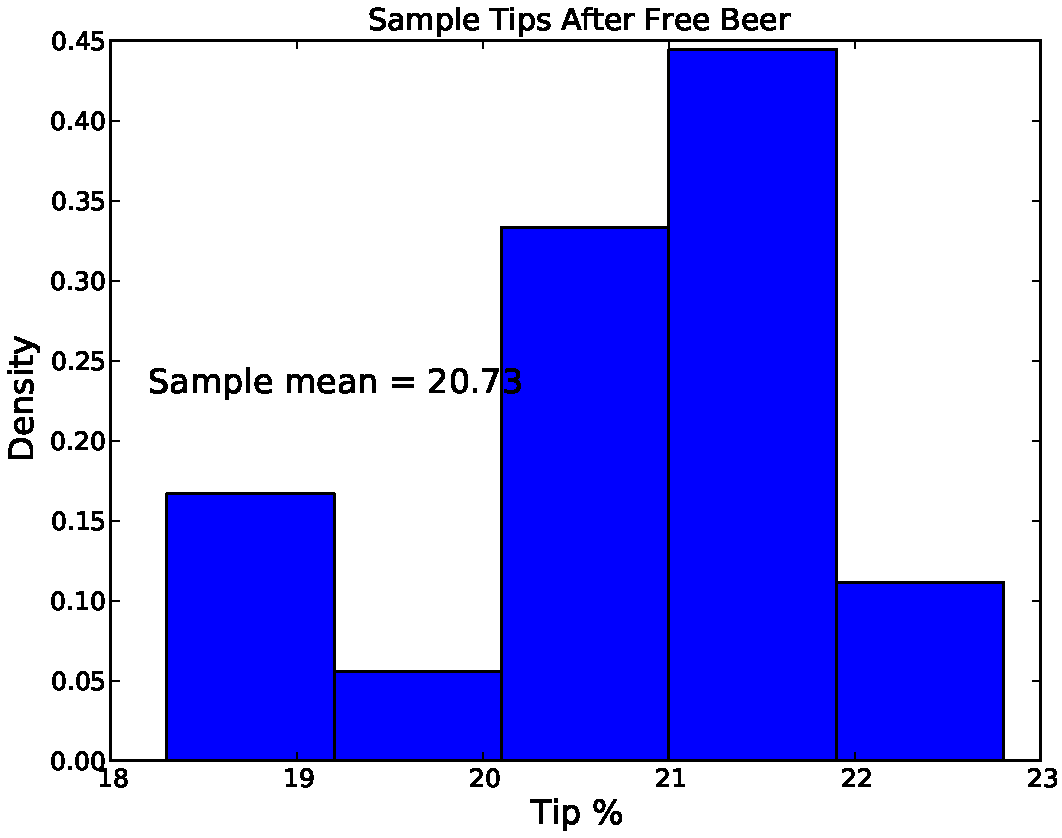
\includegraphics[width=\linewidth]{figures/tips-histo.pdf}
\caption{This is a margin figure. The helix is defined by $x = \cos(2\pi z)$, $y = \sin(2\pi z)$, and $z = [0, 2.7]$. The figure was drawn using Asymptote (\url{http://asymptote.sf.net/}).}
\label{fig:marginfig}
\end{marginfigure}

\marginnote{This is a random margin note. Notice that there isn't a number preceding the note, and there is no number in the main text where this note was written. Use \texttt{sidenote} to use a number.}

\begin{table} % Add the following just after the closing bracket on this line to specify a position for the table on the page: [h], [t], [b] or [p] - these mean: here, top, bottom and on a separate page, respectively
\centering % Centers the table on the page, comment out to left-justify
\begin{tabular}{l c c c c c} % The final bracket specifies the number of columns in the table along with left and right borders which are specified using vertical bars (|); each column can be left, right or center-justified using l, r or c. To specify a precise width, use p{width}, e.g. p{5cm}
\toprule % Top horizontal line
& \multicolumn{5}{c}{Growth Media} \\ % Amalgamating several columns into one cell is done using the \multicolumn command as seen on this line
\cmidrule(l){2-6} % Horizontal line spanning less than the full width of the table - you can add (r) or (l) just before the opening curly bracket to shorten the rule on the left or right side
Strain & 1 & 2 & 3 & 4 & 5\\ % Column names row
\midrule % In-table horizontal line
GDS1002 & 0.962 & 0.821 & 0.356 & 0.682 & 0.801\\ % Content row 1
NWN652 & 0.981 & 0.891 & 0.527 & 0.574 & 0.984\\ % Content row 2
PPD234 & 0.915 & 0.936 & 0.491 & 0.276 & 0.965\\ % Content row 3
JSB126 & 0.828 & 0.827 & 0.528 & 0.518 & 0.926\\ % Content row 4
JSB724 & 0.916 & 0.933 & 0.482 & 0.644 & 0.937\\ % Content row 5
\midrule % In-table horizontal line
\midrule % In-table horizontal line
Average Rate & 0.920 & 0.882 & 0.477 & 0.539 & 0.923\\ % Summary/total row
\bottomrule % Bottom horizontal line
\end{tabular}
\caption{Table caption text} % Table caption, can be commented out if no caption is required
\label{tab:template} % A label for referencing this table elsewhere, references are used in text as \ref{label}
\end{table}

}

\backmatter

\printindex % Print the index at the very end of the document



\end{document}